\chapter{INTRODUÇÃO}
O estudo da lógica computacional estruturada (algoritmos), através por exemplo de disciplinas como programação, são um dos grandes desafios nos cursos de tecnologia. \\
Comprovadamente a disseminação dos conceitos da lógica estruturada é uma das sete grandes dificuldades no ensino da computação [McGettrick et al., 2005], dificuldade esta que é apontada como responsável por um grande número de reprovações e desistências em cursos [Kumar, 2003].\par

Este tipo de disciplina necessita de um acompanhamento muito próximo entre estudante e professor, relacionamento este que muitas vezes é falho, com isso alguns alunos acabam não conseguindo acompanhar o desenvolvimento dos ensinamentos. A falta de resoluções de problemas mais atrativos que está ligado diretamente a didática da aula, também torna menos estimulante e massivo o aprendizado do entendimento lógico estruturado computacional [Chen e Morris 2005], isto gera um descontentamento, evasão e reprovação nas disciplinas [Gomes 2000].\par

Uma pesquisa feita por [Crews e Ziegler 1998] verificou que estudantes que estão iniciando seus estudos em lógica computacional estruturada, cometem menos erros e se sentem mais confiantes para equacionar problemas apresentados em formas de algoritmos, quando utilizam fluxogramas.\par

A utilização de fluxogramas torna mais simples o entendimento de algoritmos, devido a forma como nosso cérebro se comporta, isto é apresentado em um estudo [Da Silva 2001]. \\
Quando nos deparamos com informações de modo textual, nosso cérebro ativa apenas a região esquerda, responsável pelo processamento lógico e textual, enquanto ao apresentar informações na forma de imagens nosso cérebro mantém ativa ambos os lados, tanto o esquerdo quanto o direito,  responsável pelo processamento visual e espacial. \par


\section{Motivação}
Atualmente ferramentas que fazem essa conversão de informações possuem um foco altamente científico (são ferramentas para documentação de códigos e ou processos) ou possuem um valor de licença muito elevado, o que dificulta o acesso a estudantes. Com isso, este trabalho de conclusão de curso visa ajudar  estudantes comprometidos ao entendimento da lógica estruturada textual, a obterem êxitos em seus estudos.
////// CITAR FERRAMETAS
\par
\label{mot}


\section{Objetivo Geral}
Com base nisto este projeto tem como proposta o desenvolvimento de uma solução gratuita, para o auxílio da disseminação lógica estruturada textual de algoritmos escritos na linguagem C através da conversão de estruturas lógicas textuais para fluxogramas. 
\par Desta forma, dada uma entrada:
\begin{figure}[h]
\centering
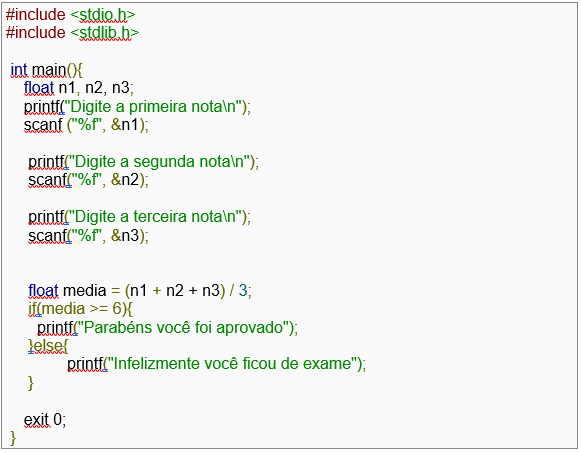
\includegraphics[width=0.9\textwidth]{figuras/Capturar.PNG}
\caption{Algoritmo em C que calcula a média de três notas}
\label{figuraEntrada}
\end{figure}

\par A ferramenta deve gerar uma saída como a abaixo.
\begin{figure}[h]
\centering
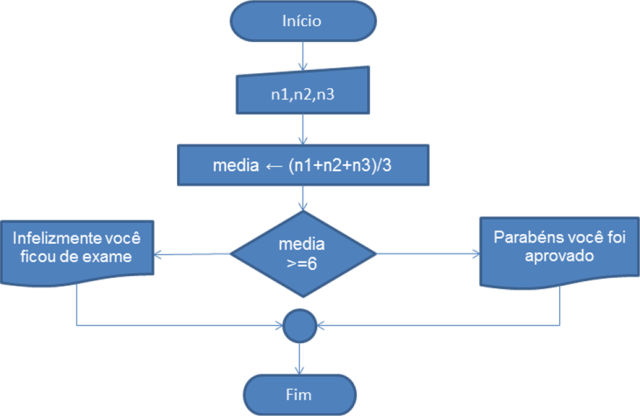
\includegraphics[width=0.9\textwidth]{figuras/fluxograma1.jpg}
\caption{Fluxograma representativo de saída}
\label{figuraSaida}
\end{figure}

\label{og}

\section{Objetivos Específicos}\label{oe}
Visando uma ferramenta totalmente gratuita e que faça a representação de uma estrutura lógica textual estruturada de forma gráfica, o objetivo deste trabalho é disposto em três etapas:
\begin{enumerate}

 \item Análise léxica e sintática necessária para separar e identificar estruturas de:
    \begin{enumerate}
    \item Entrada de dados
    \item Repetição
    \item Seleção de dados
    \item Blocos de instrução
    \item Funções
    \end{enumerate}
    
 \item Formalização das informações.
    \begin{enumerate}
    \item Após a identificação dos token (conjunto de caracteres com significado coletivo) --- REFERENCIA, seguir um modelo unificado e consolidado para representação visual das estruturas.
    \end{enumerate}
    
 \item Informações de saída.
    \begin{enumerate}
    \item Realizado o processamento e tradução dos dados é apresentado um fluxograma como especificado na etapa de formalização, assim como informações adicionais e explicativas (legendas, erros de sintaxe, erros léxicos e etc).
    \end{enumerate}
    
\end{enumerate}


\section{Justificativa}
Desenvolver a habilidade de escrever algoritmos é uma tarefa difícil, fato esse evidenciado em [DIJKSTRA 1982], onde explica-se que escrever um algoritmo necessita de um nível de raciocínio mais elevado que qualquer outra atividade. Pois também se trata de um trabalho de engenharia, devido a produção de ativos que devem seguir regras de qualidade e serem susceptíveis a apuração.\par
Assim a construção de uma ferramenta que explique esses conceitos de forma gráfica, ajudaria na compreensão de um conceito complexo e que constatadamente não possui entendimento rápido a partir de referências textuais (livros, artigos e demais formas de textuais).
\label{just}


\section{Método}
\par Tendo como um dos objetivos a acessibilidade, esta ferramenta deve ser capaz de ser executada tanto de forma online como offline. 
Com isto ela deve ser desenvolvida em uma versões web e desktop, sendo que a versão desktop poderá ser executada em sistemas Windows, Linux e Mac, visando alcançar o máximo de ambientes possíveis.
\par Com esta necessidade abordada a ferramenta deve ser desenvolvida em uma framework que adote o conceito de cross building também conhecido como cross compiler.
Pratica essa permite que um mesmo código seja utilizado para gerar uma aplicação executável em ambientes diferentes, para que o desenvolvimento ganhe produtividade e um bom grau de manutenibilidade. 
\par Assim as linguagens adotadas seram Html, css e js, através de um projeto NodeJs com React que na versão desktop será apresentado ao usuário por meio da biblioteca electron.
\par Para criação do fluxograma, os padrões especificados pelo diagrama de flowchart serão adotados, por se tratar de um modelo que possui estruturas representativas análogas as estruturas da lógica computacional estruturada textual, como:
\begin{itemize}
\item Entrada e saída de dados
\item Estruturas de repetição
\item Seleção de dados
\item Início e fim
\end{itemize}
\par Dentre outras que serão explanadas nos capítulos subsequentes.



